\cxset{
 name=CHAPTER,
 numbering=arabic,
 number font-size=large,
 number position=rightname,
 chapter spaceout=soul,
 chapter color=black,
 chapter font-size=large,
 chapter before=\hrule\vskip1pt\hfill,
 chapter after=,
 number before=,
 number after=\hfill\hfill\vskip1pt\hrule\vskip0pt\par,
 chapter margin left=0pt,
 number color=black,
 title font-family=bfseries,
 title font-color=black,
 title font-weight=,
 title font-size=Huge,
 title before=,
 title after=\par,
 title beforeskip=\vspace*{1cm},
 title afterskip=,
 title margin bottom=1.5cm,
 title margin-left=0pt,
 chapter title width=0.8\textwidth,
 chapter title align=centering,
 epigraph width=0.85\textwidth,
 epigraph align=center,
 header style=empty,
 epigraph rule width=0pt,
 section font-weight=bold}

\debugtitle
\chapter{The Chomskyan Revolution, Introduction to Style Fifty Two}

\epigraph{In the late forties \ldots\ it seemed to many that the conquest of syntax finally lay open before the profession. At the beginning of the fifties confidence was running high.}{--H. Allan Gleason}

\section{Looking for Mr. Goodstructure}

\lorem
\begin{figure}[ht]
\centering
\fbox{%
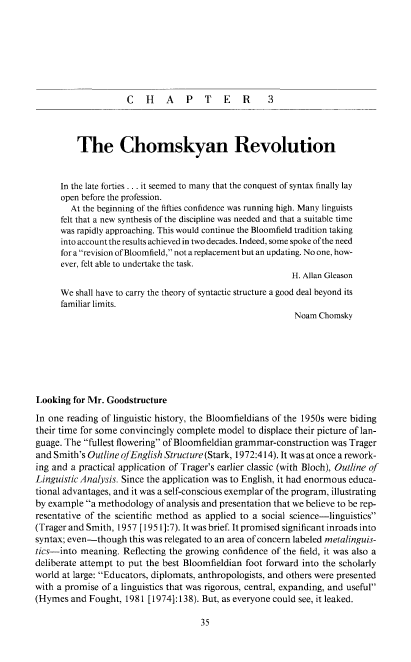
\includegraphics[width=0.35\textwidth]{./chapters/chapter52.png}
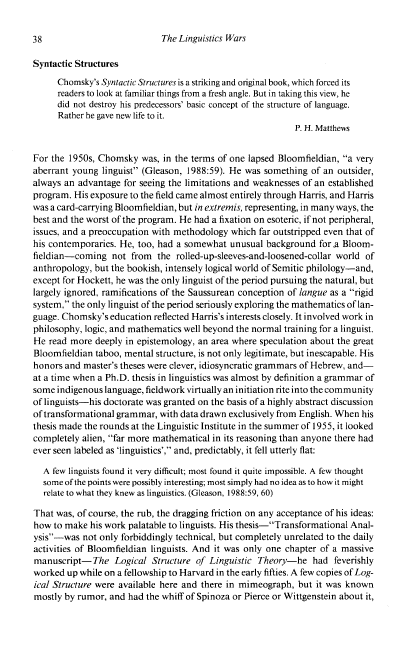
\includegraphics[width=0.35\textwidth]{./chapters/chapter52a.png}}

\caption{Style 50 from the Oxford Handbook of Cuneiform Culture.}
\end{figure}

This style is very modern and typical of many computer books. The difficulty is in integrating all the page elements to make it work flawlessly.
